\documentclass[12pt,a4paper]{article}
\usepackage{graphicx}
\usepackage{enumitem}
\newlist{steps}{enumerate}{1}
\setlist[steps, 1]{label = Step \arabic*:}

\usepackage{xcolor}
\usepackage[export]{adjustbox}
\begin{document}

\setcounter{page}{1}
\pagenumbering{roman}

\section*{Abstract}

IP convention needs the assistance of distinguishing sending blunder and control messages since it doesn't have an inbuilt component, the utilization of 
ICMP has been presented, which has utilized by network gadgets as a supporting convention. The examination objective is to show the setup of ICMP, 
interfacing two switches and confirm ICMP and utilizing 
ICMP to test the Network which neglected to arrive at the worker and right its organization availability. The examination will be performed by utilizing the Cisco Packet Tracer.

\textit{\textbf{Keywords}}: ICMP, IP,Ping,Trace,Cisco packet tracer

\pagebreak
\tableofcontents
\pagebreak

\addcontentsline{toc}{section}{List of figures}
\listoffigures
%\thispagestyle{empty}
\pagebreak

\pagebreak

\pagenumbering{arabic}
\setcounter{page}{1}
{
\centering
\section{\Large{INTRODUCTION}}
}
\subsection{Internet Protocol}
The underneath Figure for example Fig. no. 1. relates the web convention stack and the OSI reference convention. The Internet convention stack gives an association arranged solid branch (TCP) and a connectionless, untrustworthy branch (UDP) expand on top of the Internet Protocol.\\
 \begin{figure}[h]
 		\centering
				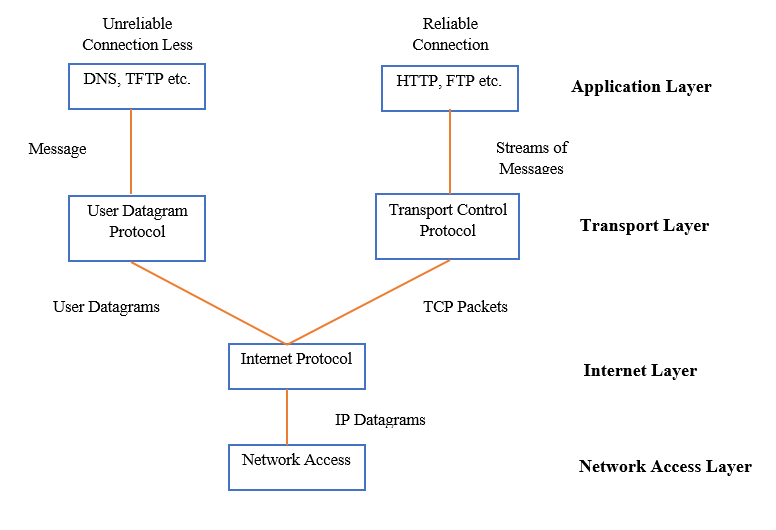
\includegraphics[scale=0.75]{1.1.png}	
			\caption{Internet Protocol Stack.}
			\label{fig:AP}
	\end{figure}
All actual execution subtleties are covered up underneath the IP layer. The IP layer gives a problematic, connectionless conveyance framework. The motivation behind why it is temperamental originate from the reality the convention doesn't give any usefulness to blunder recuperating for datagrams that are either copied, lost or show up at the far off have in another request than they are sent. On the off chance that no such blunders happen in the actual layer, the IP convention ensures that the transmission is ended effectively. 
The essential unit of information trade in the IP layer is the Internet Datagram. The organization of an IP datagram and a short portrayal of the main fields are remembered for Fig. no. 2.:\\
\begin{figure}[h]
 		\centering
				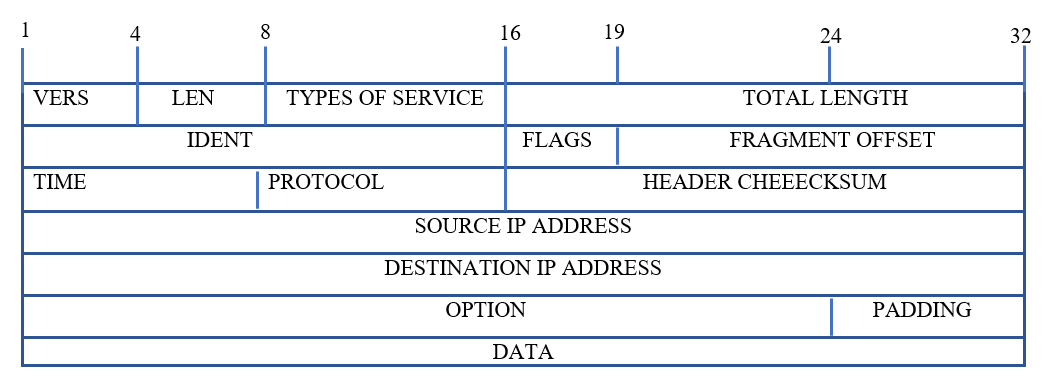
\includegraphics[scale=0.65]{1.2.png}	
			\caption{Internet Protocol Datagram.}
			\label{fig:AP}
	\end{figure}
 
 \begin{enumerate}
\item LEN: The number of 32 bit-segments in the IP header\\
\item TYPES OF SERVICE: Each IP datagram can be given a precedence value ranging from 0-7, showing the importance of the datagram. This is to allow out-of-band data to be routed faster than normal data. \\
\item IDENT, FLAGS AND FRAGMENT OFFSET: These fields are used to describe the fragmentation of a datagram. \\
\item TIME: This is the remaining Time To Live (TTL) for a datagram when it travels on the Internet.\\
\item SOURCE IP-ADDRESS AND DESTINATION IP-ADDRESS: Both the source and the destination address is indicated in the datagram header so that the recipient can send an answer back to the transmitting host.
\end{enumerate}
 \pagebreak
\subsection{ICMP}
ICMP is designed to overcome the following two problems with IP Protocol\\
 \begin{enumerate}
\item No Error reporting(Correcing mechanism)
\item Lacks a mechanism for queries
\end{enumerate}

It is a network layer protocol, but its msg are not passed to the data link layer. Its msg are first encapsulated inside an IP datagram before going to the lower layer.\\

ICMP position is shown in below  Fig. no. 3. 
\begin{figure}[h]
 		\centering
				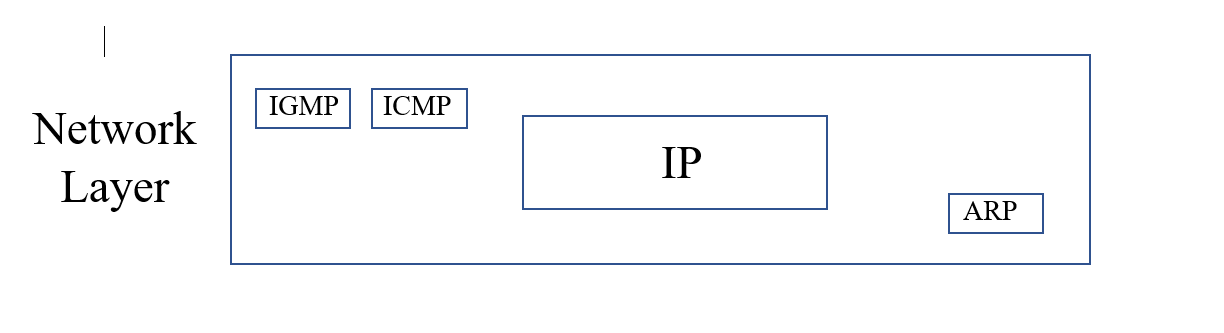
\includegraphics[scale=0.5]{1.3.png}	
			\caption{ICMP position.}
			\label{fig:AP}
	\end{figure}
ICMP messages are not directly passed to the Data link layer. The message is first encapsulated inside IP datagrams before going to the lower layer.
\begin{figure}[h]
 		\centering
				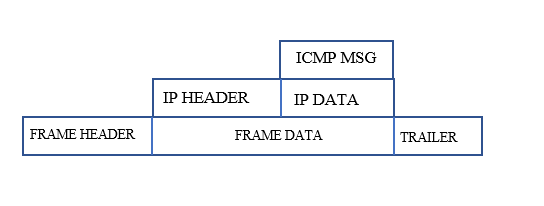
\includegraphics[]{1.4.png}	
			\caption{ICMP Encapsulation.}
			\label{fig:AP}
	\end{figure}
\subsubsection {ICMP message}
Two type of messages in ICMP:
 \begin{enumerate}
\item ERROR REPORTING: They report problem that are router or a host may encounter whille processing of IP pocket.
\item QUERY: Fetch important/specific information from a router or host.
\end{enumerate}

 
\subsubsection {ICMP message format}
\begin{figure}[h]
 		\centering
				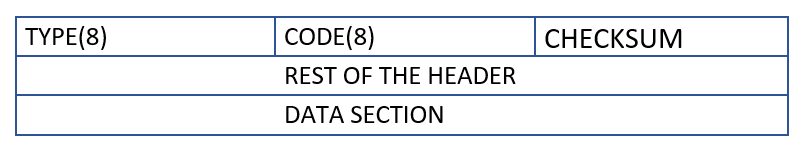
\includegraphics[scale=0.75]{1.5.png}	
			\caption{ICMP Format.}
			\label{fig:AP}
	\end{figure}
 \begin{enumerate}
\item TYPES: Defines the msg type
\item CODE: Reason for  message type 
\item CHECKSUM: Error Checking
\item REST OF HEADER: Specified for each msg type
\item DATA SECTION: Find the original packet with error.for queries it carries extra infomartaion.
\end{enumerate}
\pagebreak

\section{\Large{IMPLEMENTATION SETUP}}
\subsection{Cisco Packet Tracer}
Packet Tracer is a cross-platform visual simulation tool designed by Cisco Systems that allows users to create network topologies and imitate modern computer networks. The software allows users to simulate the configuration of Cisco routers and switches using a simulated command-line interface.
\begin{steps}
  \item Go to the website www.netacad.com
\begin{figure}[h]
 		\centering
				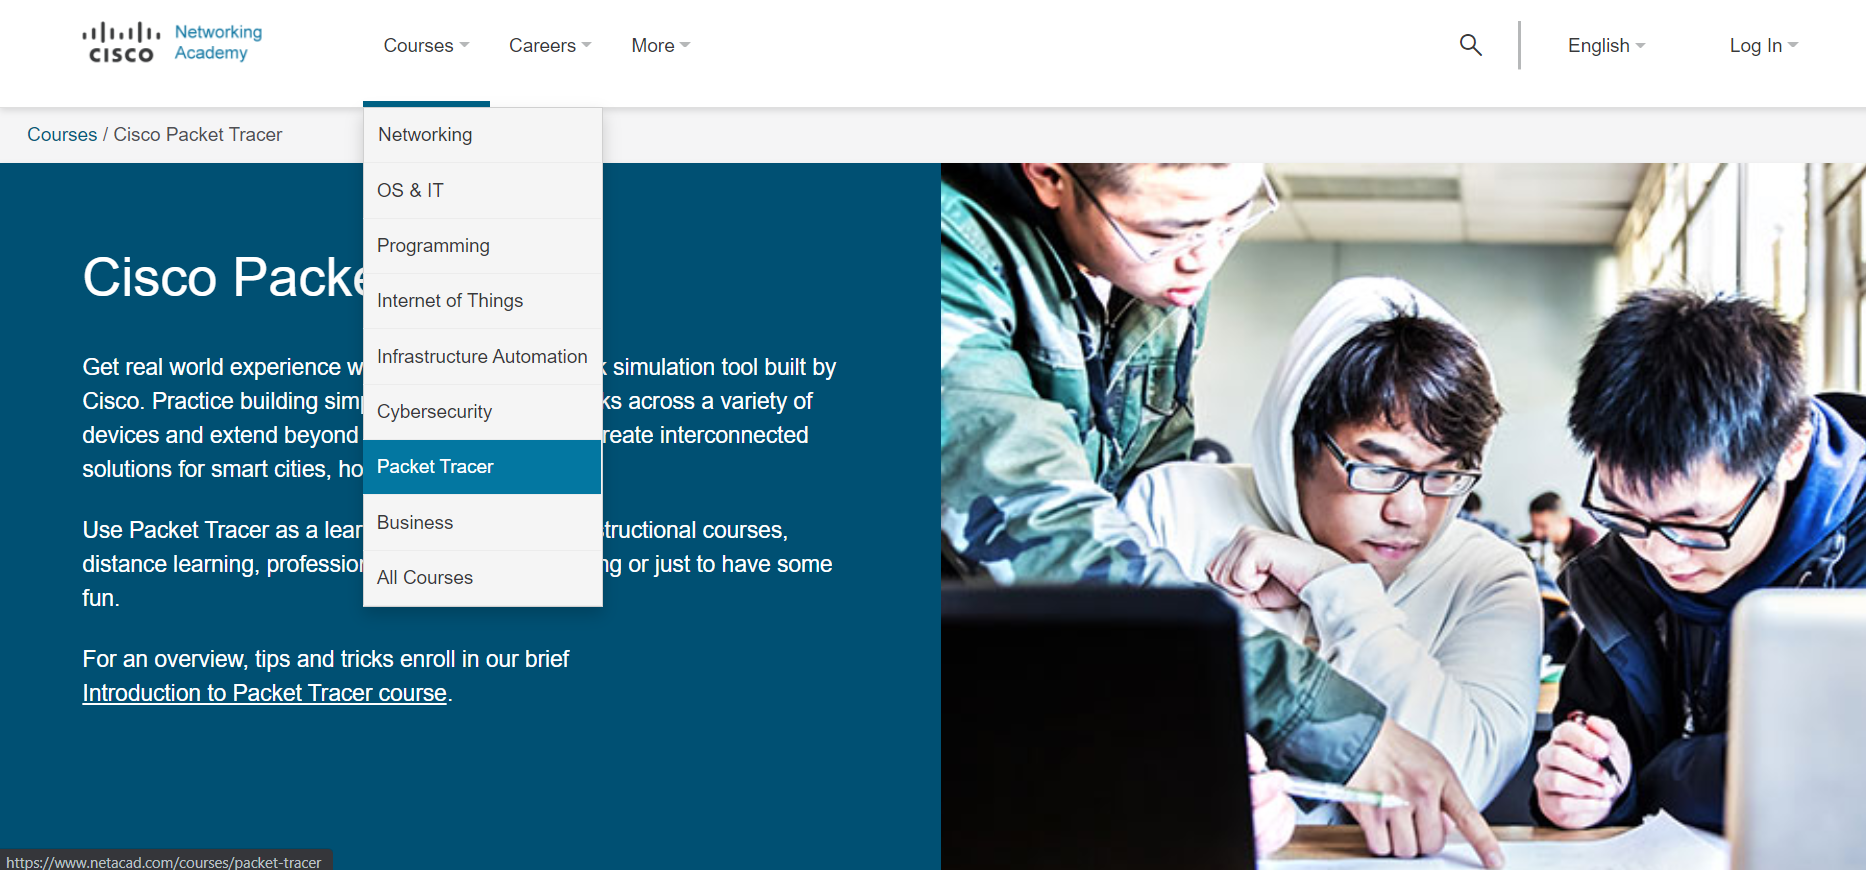
\includegraphics[scale=0.20]{2.1.png}	
	\end{figure}
  \item Click the course tab and select Packet Tracer

  \item Click on the learn more button in  the course intro to packet tracer
	

\item Create an account 

\item After redirecting to new page, click on resources tab and download Packet Tracer
\begin{figure}[h]
 		\centering
				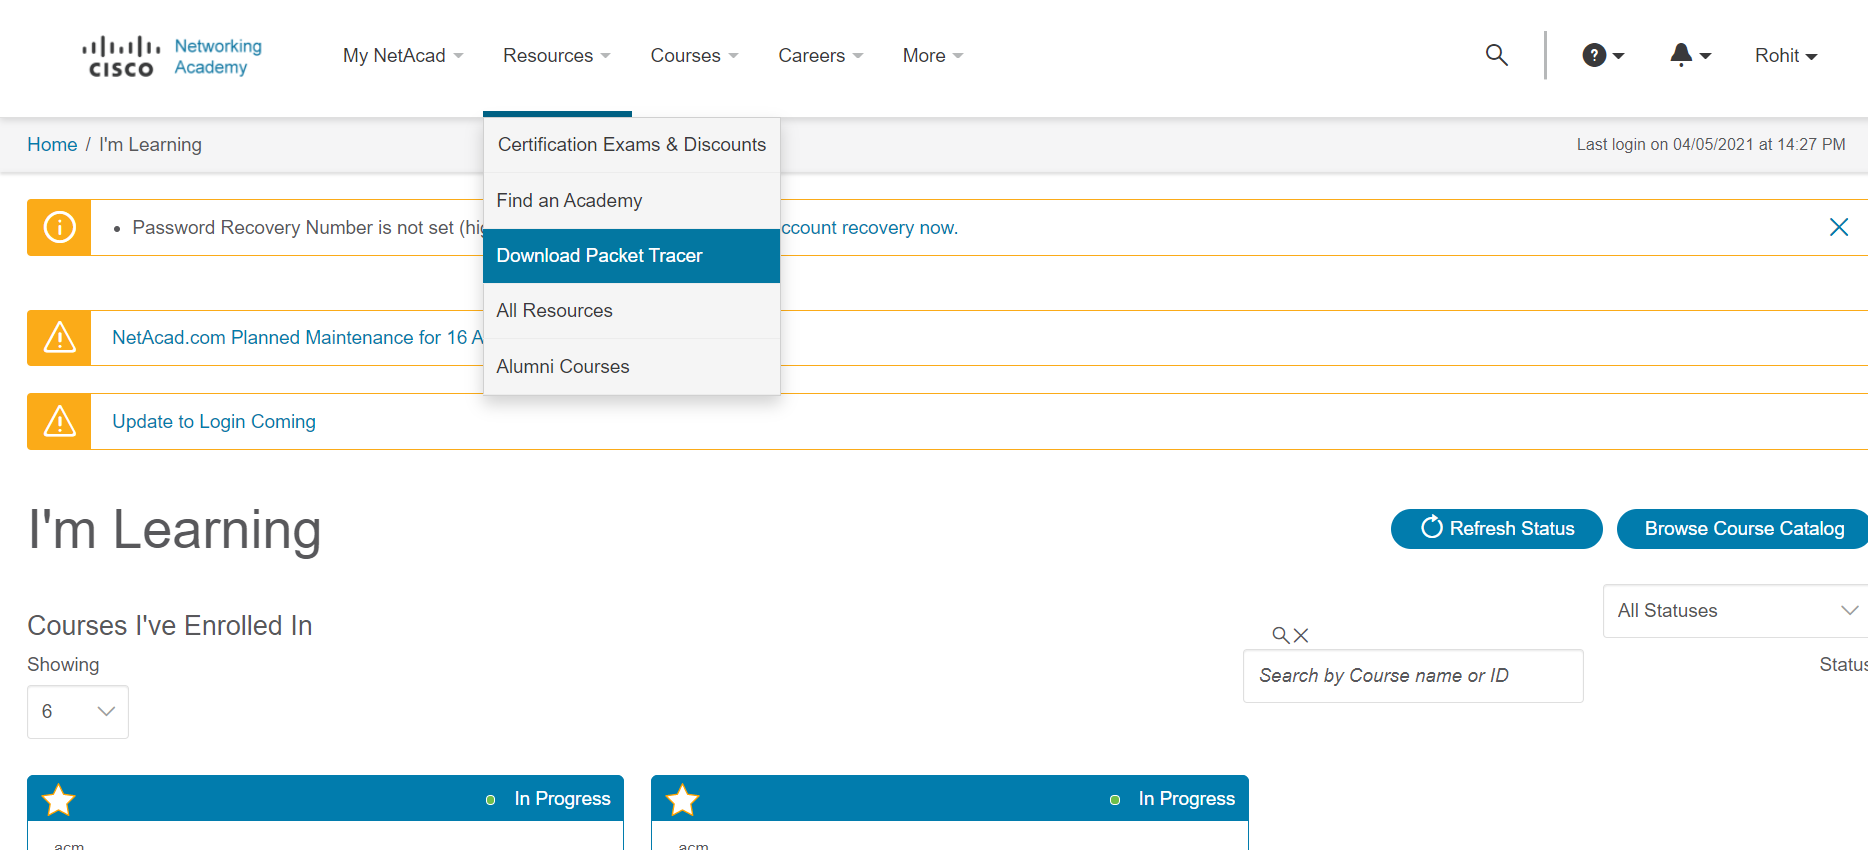
\includegraphics[scale=0.19]{2.8.png}	
	\end{figure}
\item Download the version according to your system
\pagebreak
\item Cisco Packet Tracer is ready to start the project
\begin{figure}[h]
 		\centering
				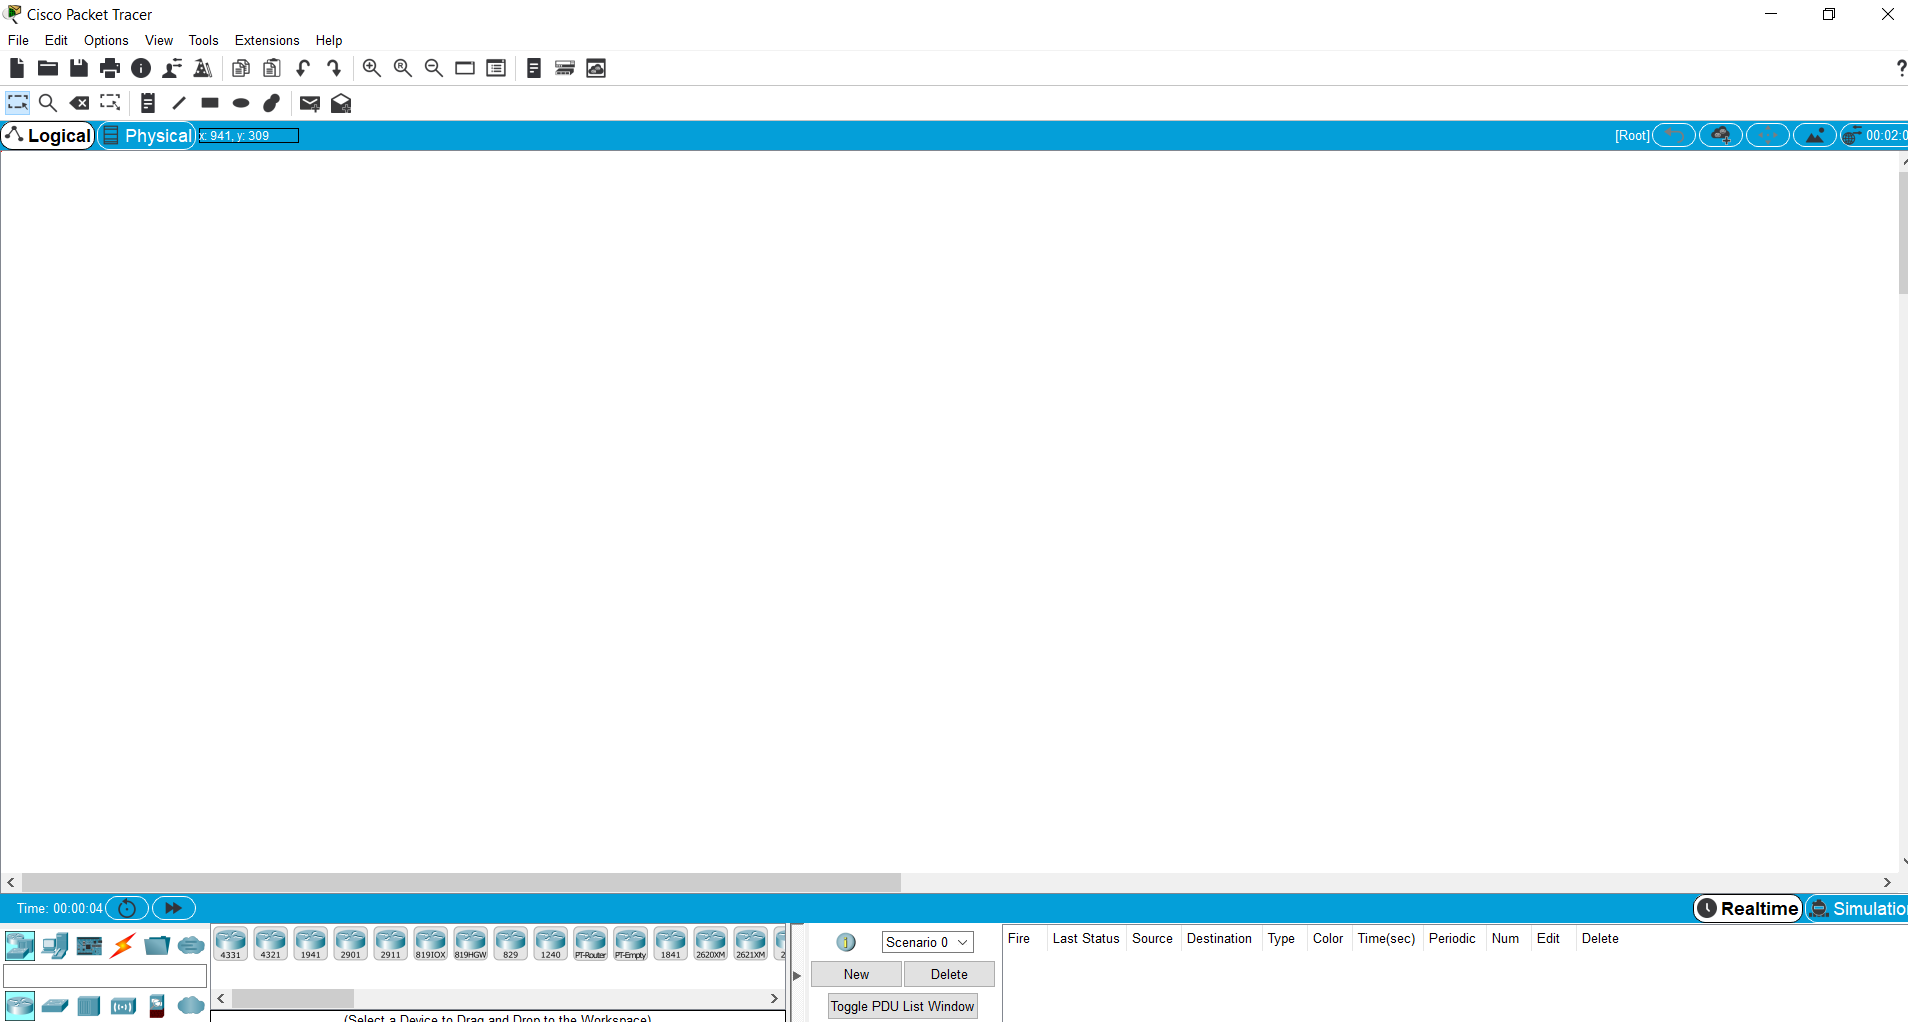
\includegraphics[scale=0.19]{2.10.png}	
	\end{figure}
\end{steps}
\subsection{Wireshark}
Wireshark is a free and open-source parcel analyzer. It is utilized for network investigating, examination, programming and interchanges convention improvement, and training.
\begin{steps}
  \item Go to the website www.wireshark.org/download.html

\item Download the software according to your system
\item Wireshark is ready to start

\begin{figure}[h]
 		\centering
				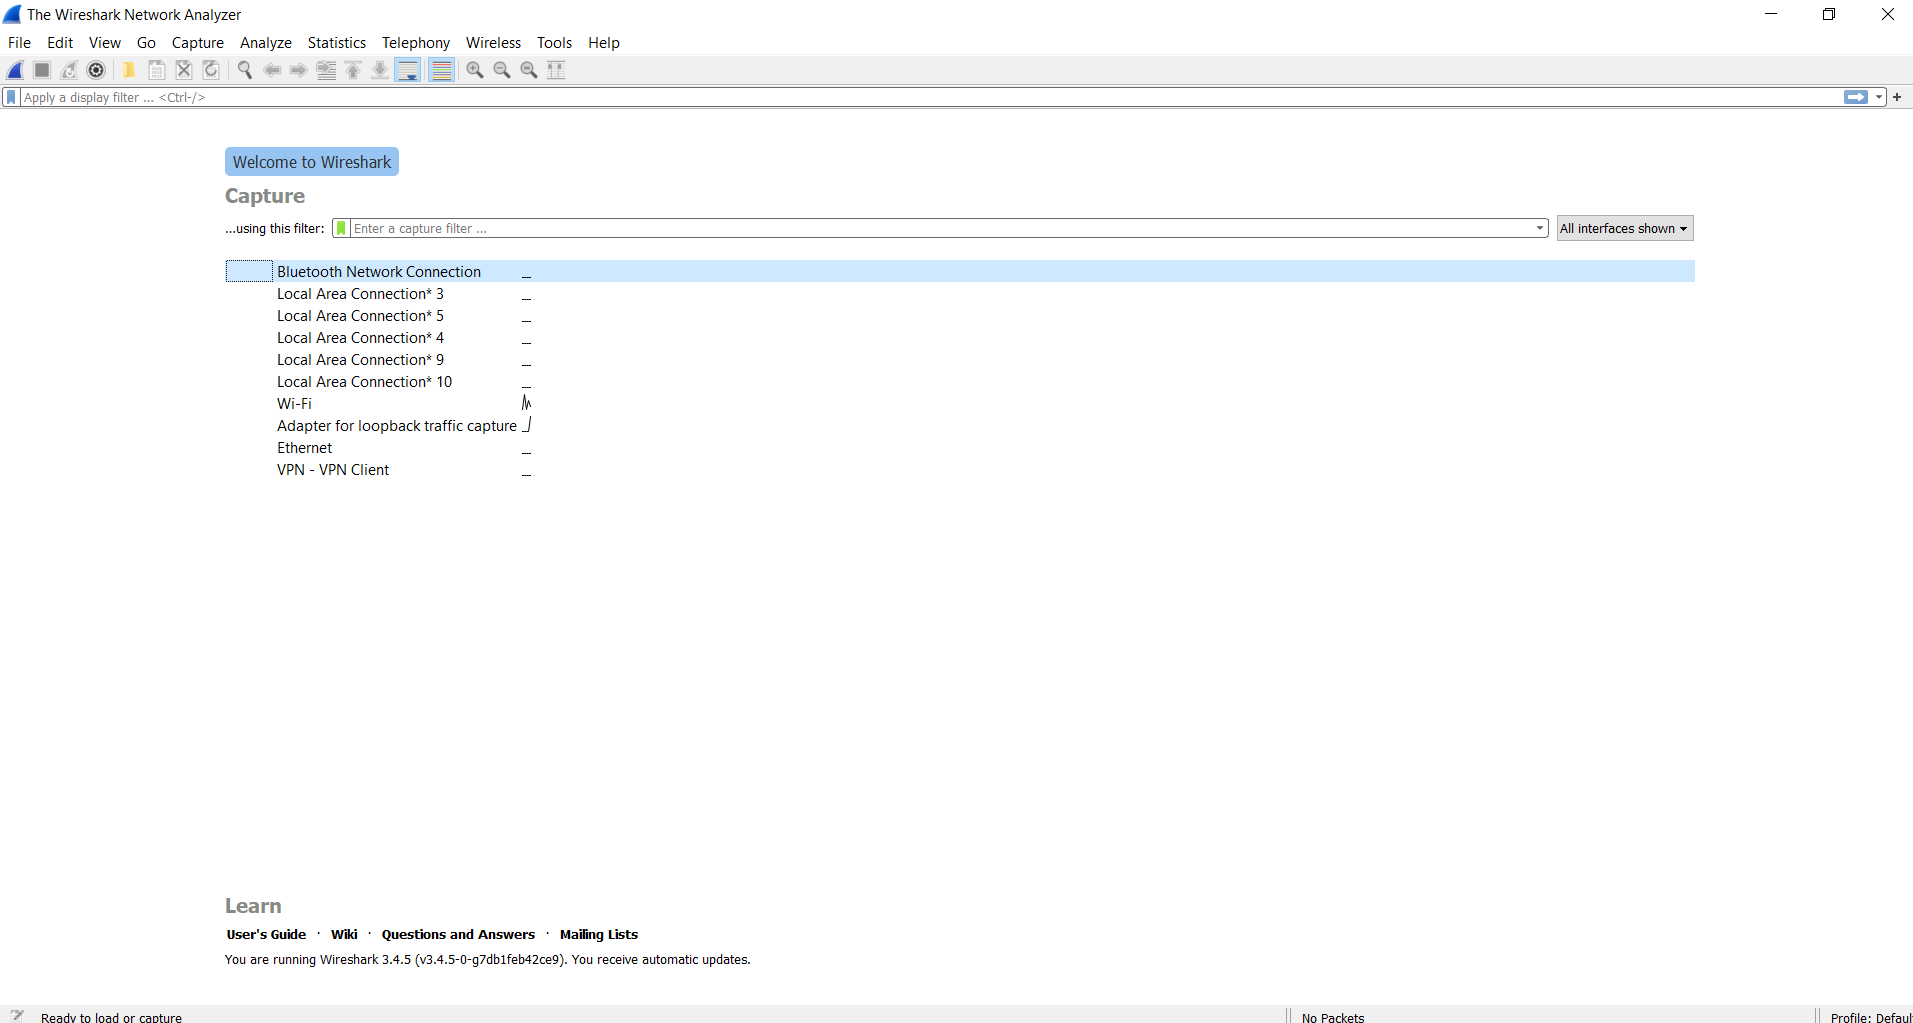
\includegraphics[scale=0.25]{6.2.png}	
				
	\end{figure}
\end{steps}
\pagebreak
\section{\Large{IMPLEMENTATION}}
\subsection{ICMP Configuration }

ICMP Protocol is generally used for troubleshooting activities. The main two troubleshooting commands for network engineers are “ping” and “traceroute” that works with Internet Control Message Protocol .\\

Ping is a utility used in computer network administration software to test the reachability of a host on an Internet Protocol (IP) network.\\

In the cisco packet tracer environment, we create a network that is shown in Fig. no. 6.
\begin{figure}[h]
 		\centering
				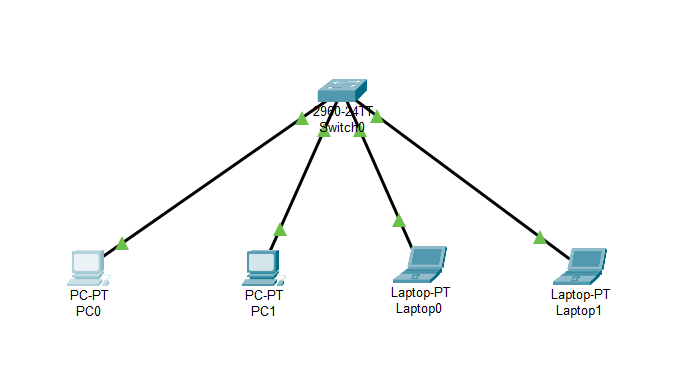
\includegraphics[scale=0.75]{3.1.png}	
			\caption{ICMP Configuration.}
			\label{fig:AP}
	\end{figure}

The 4 devices are connected with a switch and we assigned there stactic IP addresses   and subnet masks.
\begin{figure}[h]
 		\centering
				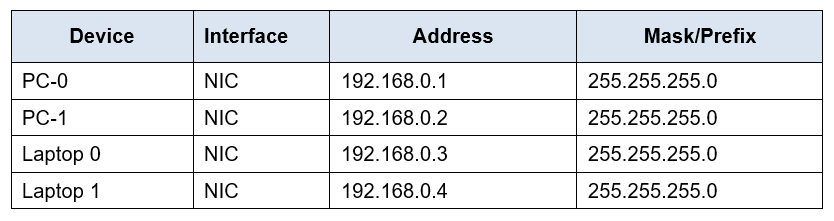
\includegraphics[scale=0.75]{3.2.png}	


			\caption{IP address configuration.}
			\label{fig:AP}
	\end{figure}
\\Pinging from PC-0 to the other three systems is giving us a response as shown in Fig. No. 8. so that means the message can be sent among the system through the switch and has been checked by using ICMP protocol.
\begin{table}[h!]
\begin{center}
\centering
\caption{Addressing table.}
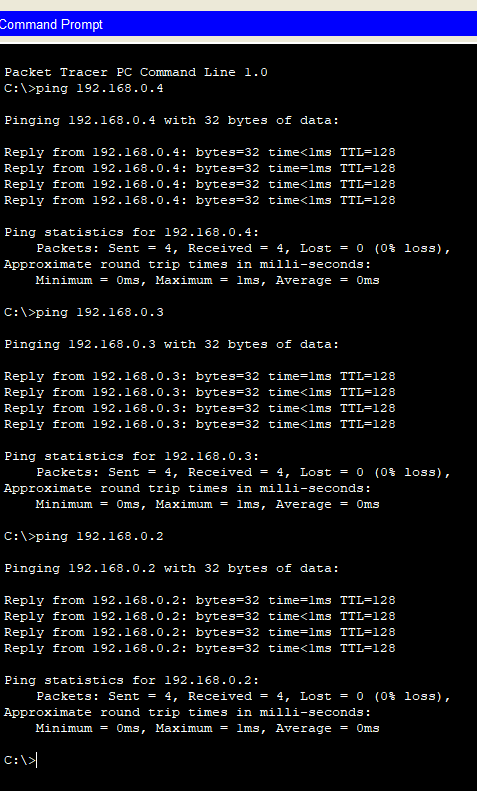
\includegraphics[scale=0.75]{3.3.png}	
\end{center}
\end{table}
\pagebreak
\subsection{Connect two router and verify ICMP}
In this experiment, there are 4 systems, 2 switch and 2 routers, as shown in Fig. No. 9. Two systems have been assigned with class A IP configuration, and the other two has been with class C configuration, and we are going to connect the class A and class C network and ping it.

\begin{figure}[h]
 		\centering
				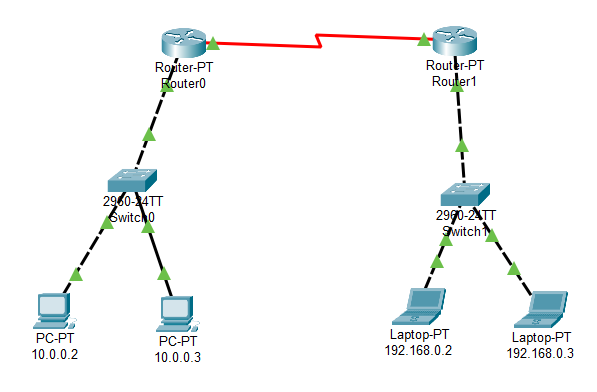
\includegraphics[scale=0.75]{4.1.png}	


			\caption{Experiment  connection.}
			\label{fig:AP}
	\end{figure}
The IP addresses, the subnet mask and the default gateway has been configured as shown in the table no. 2.
\begin{table}[h!]
\begin{center}
\centering
\caption{Addressing table.}
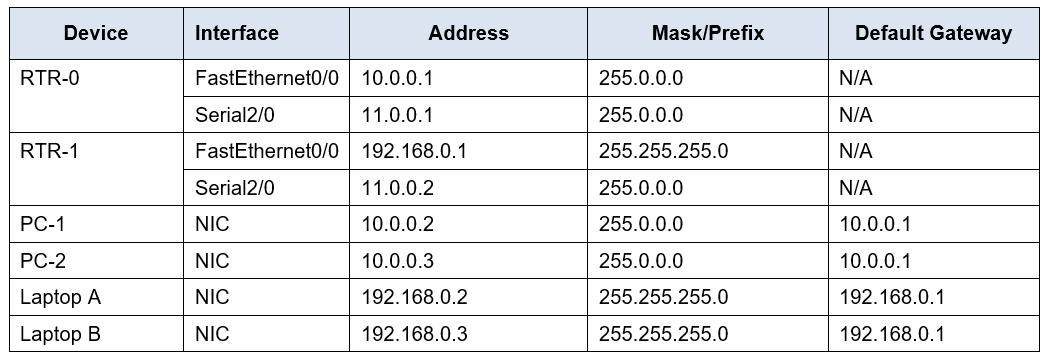
\includegraphics[scale=0.65]{4.2.png}	
\end{center}
\end{table}
\pagebreak
Running the ping command from the 10.0.0.2 to 192.168.0.2 we successfully get the response as shown in Fig. no. 10.\\
\begin{figure}[h]
 		\centering
				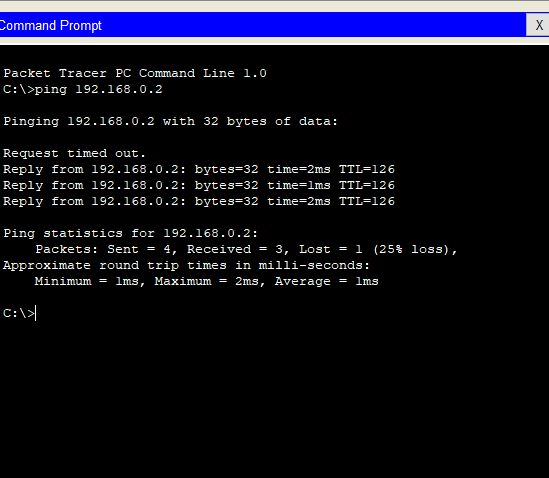
\includegraphics[scale=0.75]{4.10.png}	


			\caption{Pinging to system.}
			\label{fig:AP}
	\end{figure}
\pagebreak
\subsection{Use ICMP to  test and correct network connectivity}
In this experiment, ICMP is used to test network connectivity and locate network problems and to correct simple configuration issues and restore connectivity to the network.\\

\begin{table}[h!]
\begin{center}
\centering
\caption{Addressing table.}
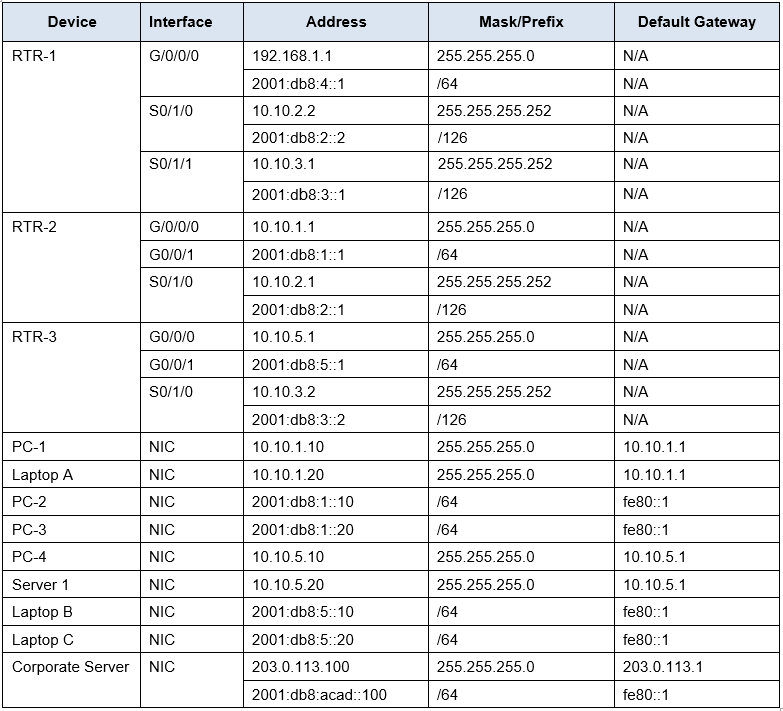
\includegraphics[scale=0.75]{5.13.png}	
\end{center}
\end{table}
\begin{figure}[h]
 		\centering
				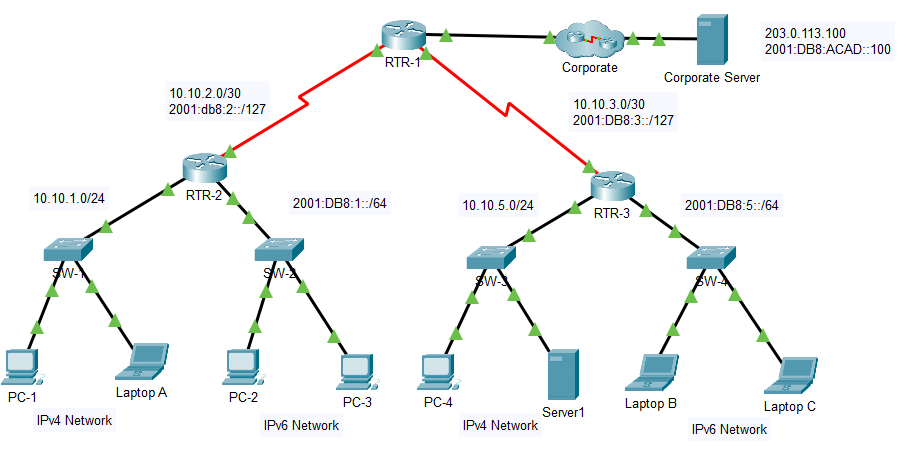
\includegraphics[scale=0.75]{5.1.png}	


			\caption{Experiment network connectivity.}
			\label{fig:AP}
	\end{figure}
The addressing table of the given network is shown in Fig. no. 12, and in Fig. no. 11 it shows the connection, and there is some error in that some devices are unreachable from the corporate server, and our objective is to find that and restore the connectivity with the help of ping and trace with comparison to the addressing table.\\
\pagebreak\\
Pinging to corporate server(IPv4:203.0.113.100 or IPv6:2001:db8:acad::100 ) from all the devices let us know which is unreachable.

First of all, for PC-1 of IPv4 address, we get a response from the server and again from Laptop-A of IPv4 address, we also get a response.

Next, we ping from PC-2 and PC-3 of IPv6 addresses we get a response.

Next, we ping from PC-4 of IPv4 address, but we don't get a response as shown in Fig. no. 11. \\
\begin{figure}[h]
 		\centering
				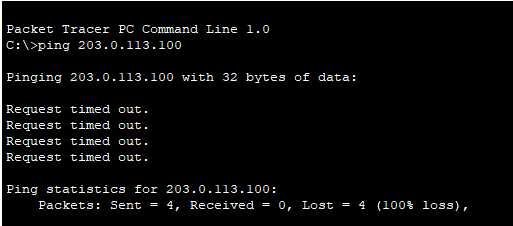
\includegraphics[scale=0.75]{5.2.png}	


			\caption{Ping not response from PC-4 to coperate server.}
			\label{fig:AP}
	\end{figure}
\pagebreak \\
So, we will trace and identify the problem as shown in Fig. no. 12. Tracert is commands that display possible paths and measuring transit delays of packets across an IP network.

\begin{figure}[h]
 		\centering
				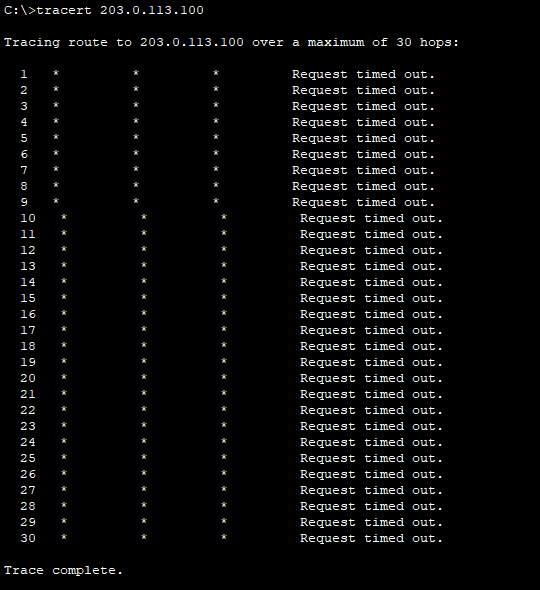
\includegraphics[scale=0.75]{5.3.png}	


			\caption{Tracing.}
			\label{fig:AP}
	\end{figure}
Now, we know that it didn't go to its default gateway.
So, we verify PC-4 with its addressing table, and now we get to know that the default gateway is 10.10.5.11 instead of 10.10.5.1. Now replace with correct default gateway as shown in Fig. No. 13.\\
\begin{figure}[h]
 		\centering
				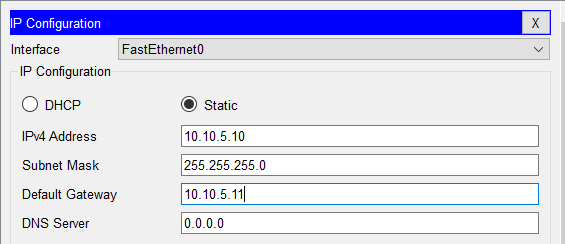
\includegraphics[scale=0.75]{5.4.png}	


			\caption{IP configuration.}
			\label{fig:AP}
	\end{figure}
\pagebreak \\
Now, we will trace again from PC-4 and it is showing response  and get ping response as shown in Fig. no. 14.\\

\begin{figure}[h]
 		\centering
				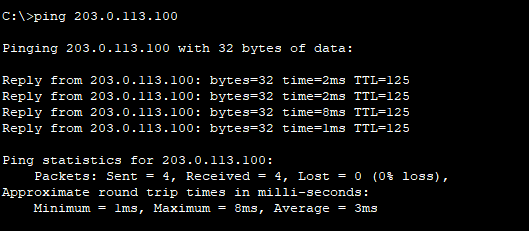
\includegraphics[scale=0.75]{5.5.png}	


			\caption{Pinging.}
			\label{fig:AP}
	\end{figure}

Next, we ping from server 1 to cooperate server, and it didn't get a response. So, we check the configuration using the command "ipconfig /all" as shown in Fig. no. 15, and we get to know that its IP address is DHCP.
\begin{figure}[h]
 		\centering
				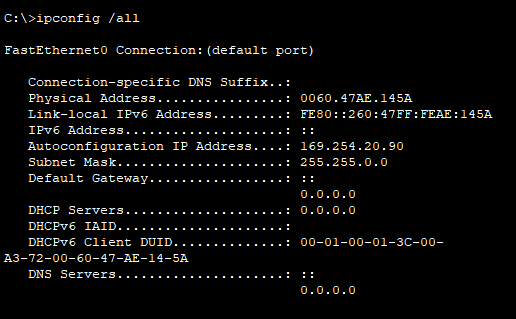
\includegraphics[scale=0.70]{5.6.png}	


			\caption{Showing IP configuration.}
			\label{fig:AP}
	\end{figure}

Now we convert it to static IP address using the adressing table as shown in Fig. no. 16.
\begin{figure}[h]
 		\centering
				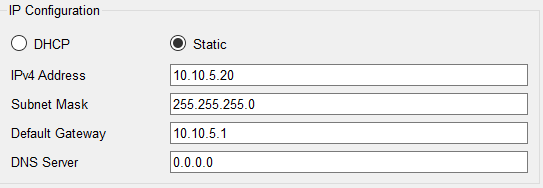
\includegraphics[scale=0.70]{5.7.png}	


			\caption{Converting to static IP.}
			\label{fig:AP}
	\end{figure} 
\pagebreak \\
 After that we again check for ping and we get the reply as shown in Fig. no. 17.\\
\begin{figure}[h]
 		\centering
				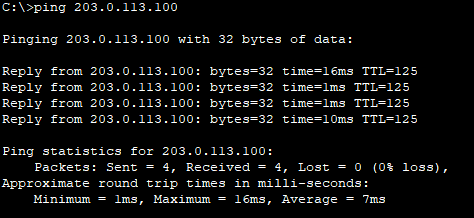
\includegraphics[scale=0.75]{5.8.png}	


			\caption{Ping response from coperate server to server 1 .}
			\label{fig:AP}
	\end{figure}
Next we go to laptop B and ping to coperate server and we didn't get a response and we used the "tracert" command to check and we found out that it didn't go to default gateway as shown in Fig. no. 18.
\begin{figure}[h]
 		\centering
				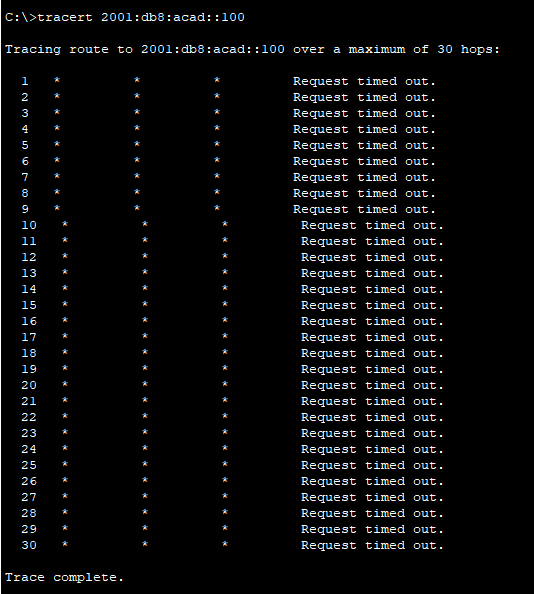
\includegraphics[scale=0.75]{5.9.png}	


			\caption{Tracing.}
			\label{fig:AP}
	\end{figure} 
\pagebreak \\
Next, we verify IP configuration with the addressing table, and we found it to be correct. Now, we go to router RTR-3 and proceed with the following command as shown in the Fig. no. 19 and we found out that IP configuration is incorrect while comparing with the addressing table.
\\
\begin{figure}[h]
 		\centering
				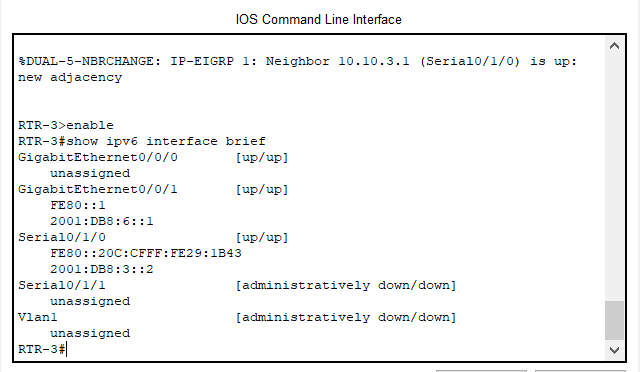
\includegraphics[scale=0.75]{5.10.png}	


			\caption{Checking IP confirugation in router.}
			\label{fig:AP}
	\end{figure}

Now we re-assigned the IP address using the follwing command as shown in the Fig. no.  20.\\
\begin{figure}[h]
 		\centering
				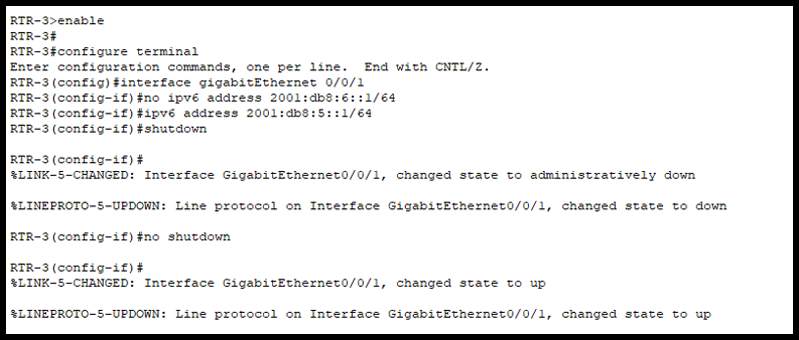
\includegraphics[scale=0.75]{5.112.png}


			\caption{Changing IP address in router.}
			\label{fig:AP}
	\end{figure}
\pagebreak \\
And now we re-do the  trace in laptop B and it got response and  ping was successfull. 
\begin{figure}[h]
 		\centering
				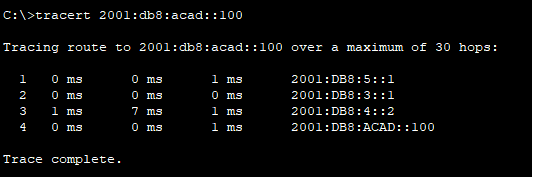
\includegraphics[scale=0.75]{5.12.png}	


			\caption{Tracing.}
			\label{fig:AP}
	\end{figure}

Finally, we check for last system laptop C and we get responsed.
\subsection{ICMP packets capture using Wireshark}
First we ping to www.google.com in the command prompt and we get a reply.As this is ICMP request packet so we can see source IP as my system IP address and destination IP as Google’s one IP address. Also IP layer mentioned the protocol as ICMP.
\begin{figure}[h]
 		\centering
				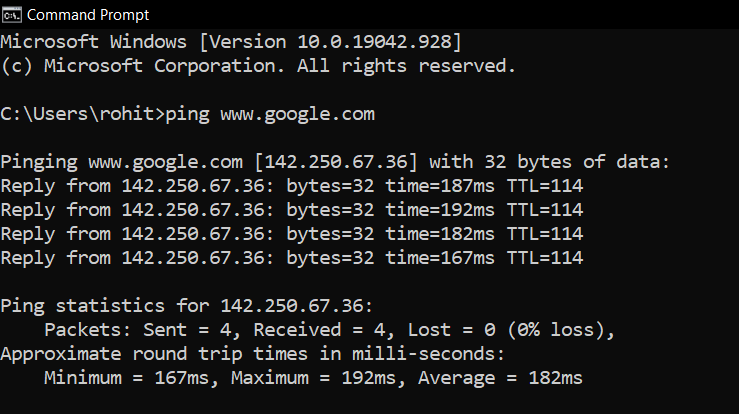
\includegraphics[scale=0.60]{6.7.png}	


			\caption{Pinging to google}
			\label{fig:AP}
	\end{figure}
\pagebreak

The same thing we can see it in wireshark as shown below figure with the ICMP message format.

\begin{figure}[h]
 		\centering
				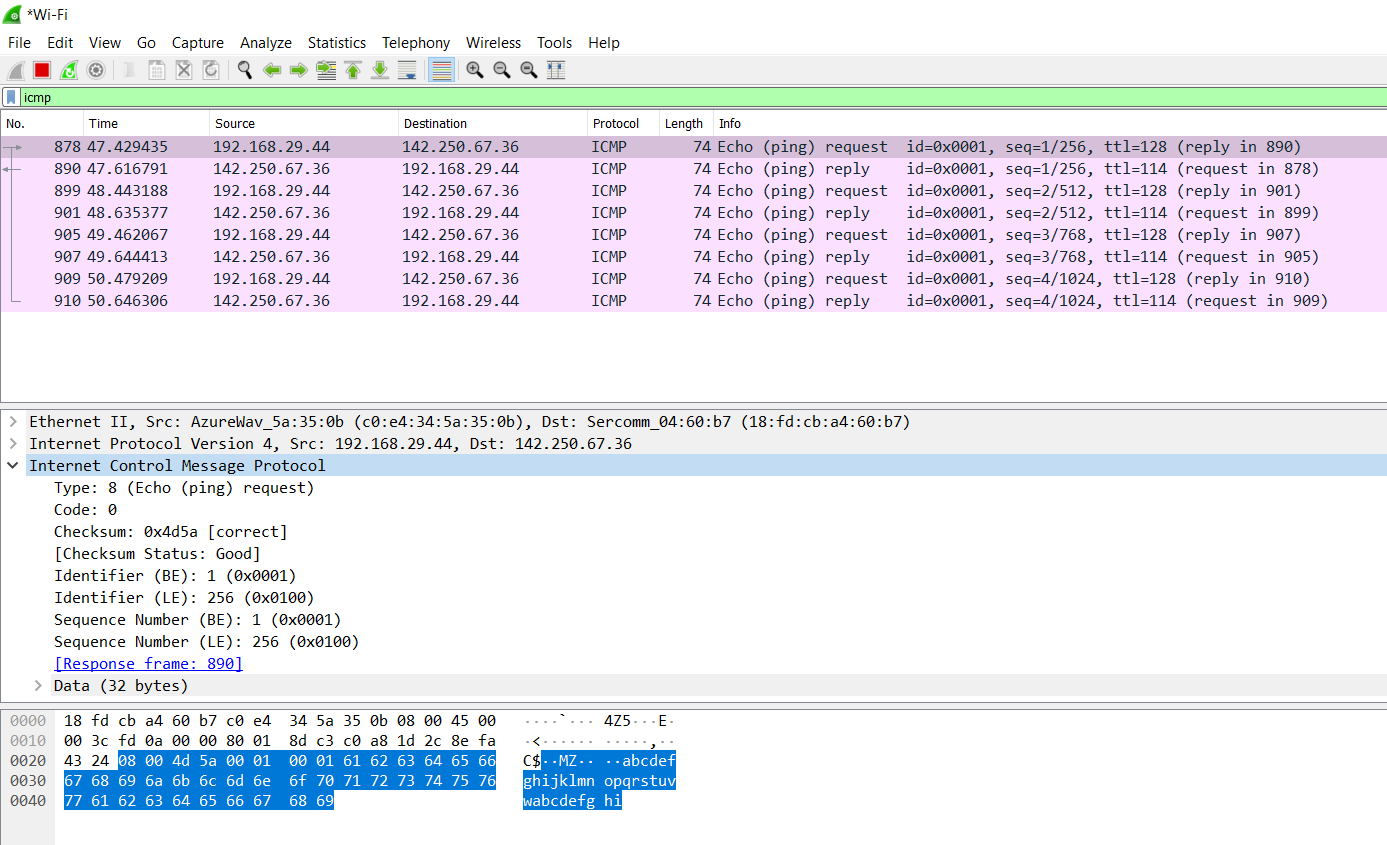
\includegraphics[scale=0.3]{6.3.png}	


			\caption{Wireshark- Pinging to google}
			\label{fig:AP}
	\end{figure}

Now we again ping to www.uom.ac.wu and we didn't get the reply as shown in below figure.

\begin{figure}[h]
 		\centering
				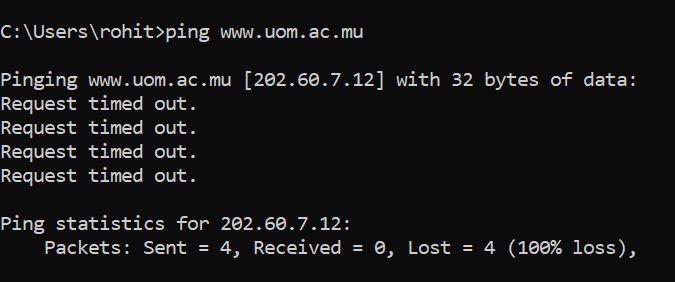
\includegraphics[scale=0.75]{6.8.png}	


			\caption{Pinging to www.uom.ac.wu}
			\label{fig:AP}
	\end{figure}

The same thing we can see it in wireshark as shown below figure 25 with the ICMP message format.
\pagebreak
\begin{figure}[h]
 		\centering
				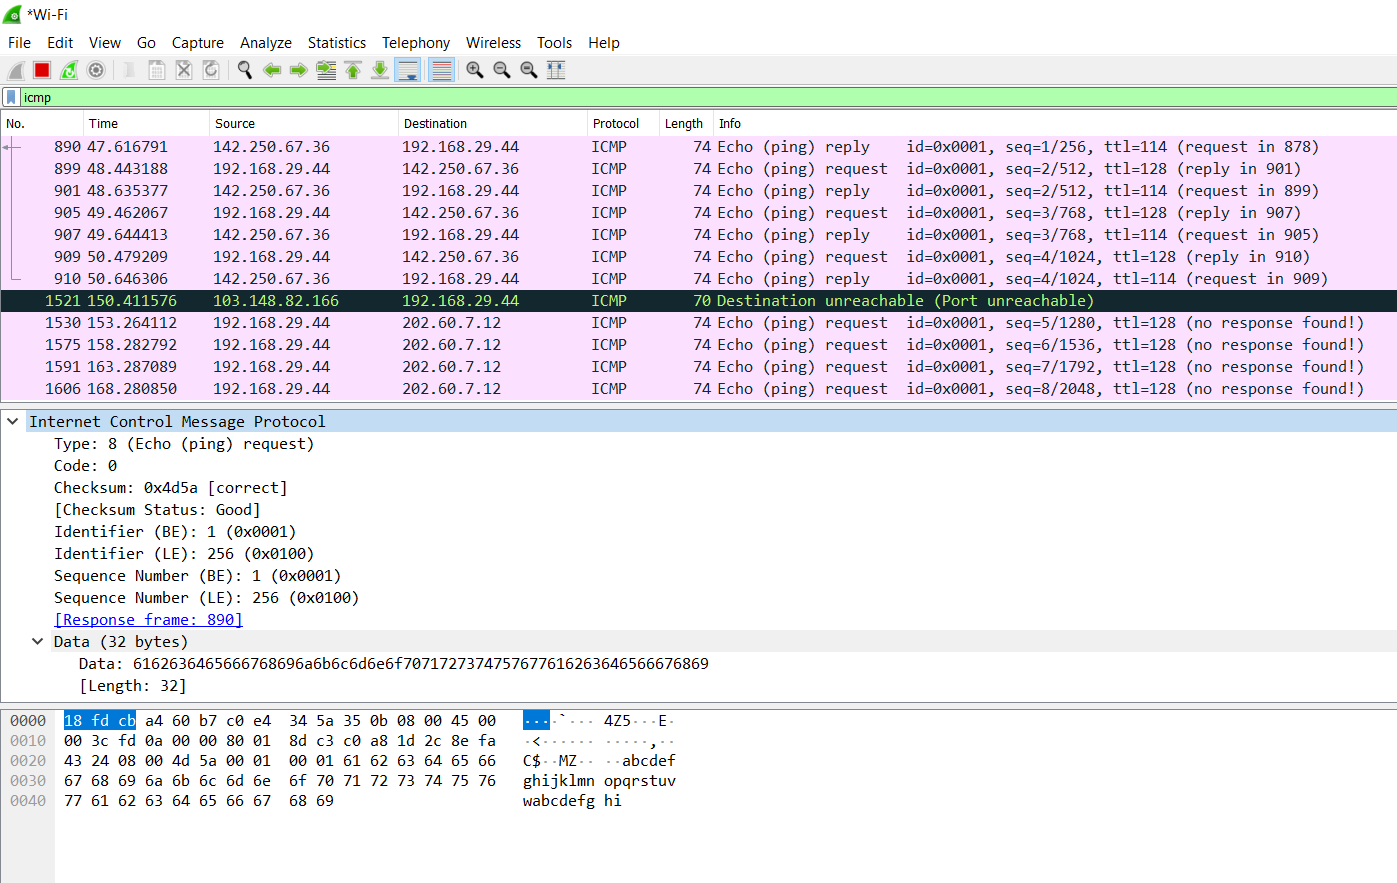
\includegraphics[scale=0.3]{6.4.png}	


			\caption{Wireshark- Pinging to www.uom.ac.wu}
			\label{fig:AP}
	\end{figure}

This doesn't mean that the server is unreachable , this means that the ICMP message were block by the firewall o the destination address.

Now, Lets us look at the TRACEROUTE  as shown in below figure.

\begin{figure}[h]
 		\centering
				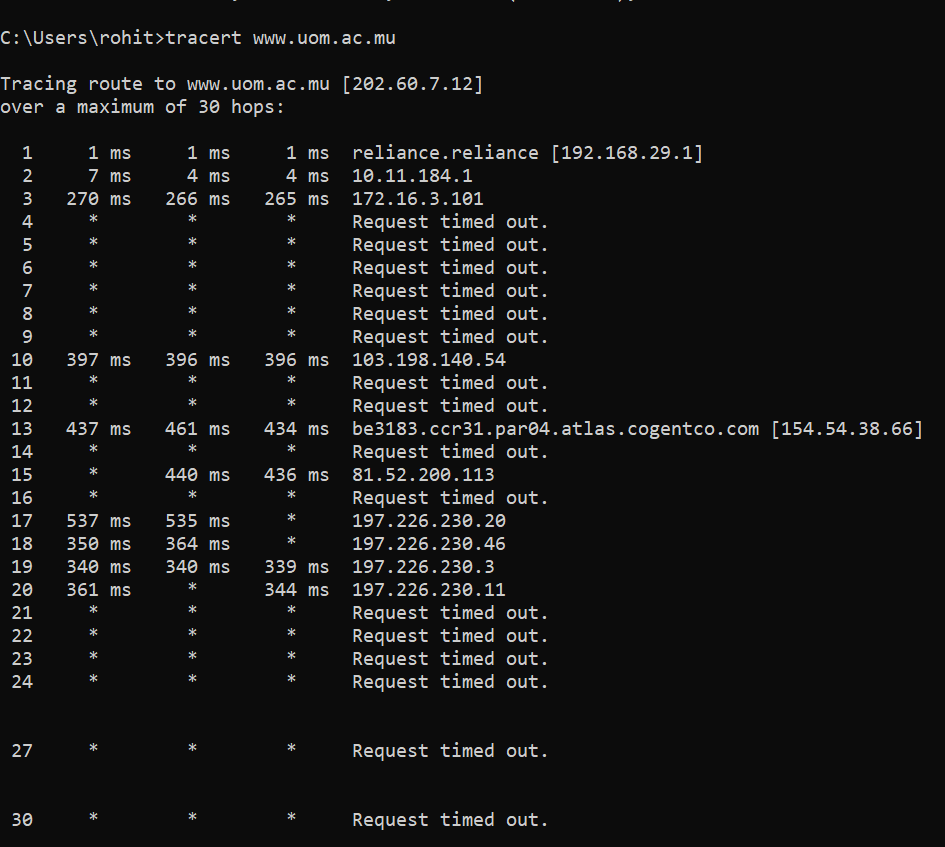
\includegraphics[scale=0.27]{6.9.png}	


			\caption{tracing to to www.uom.ac.wu}
			\label{fig:AP}
	\end{figure}
\pagebreak
The same thing we can see it in wireshark as shown below figure with the ICMP message format.

\begin{figure}[h]
 		\centering
				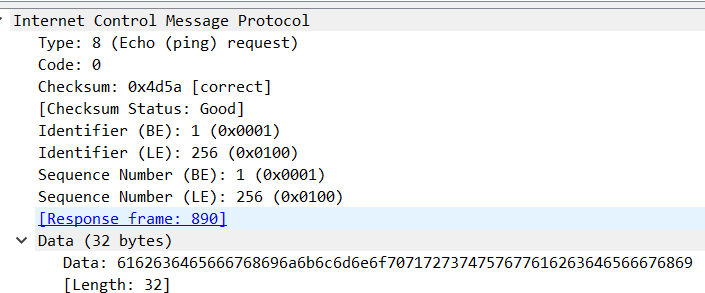
\includegraphics[scale=0.7]{6.5.png}	


			\caption{ICMP message format using Wireshark}
			\label{fig:AP}
	\end{figure}

We can see from this the ICMP has been rerturn , It has been  highlighted to show us that there as not been a response. Also it  has been prove that it can be used a diagnosed network issues.
\pagebreak
\section{\Large{Conclusion}}
We have configured ICMP , connect 2 routers and verify ICMP, Use ICMP to test and correct network connectivity, Use wireshark to show the message formate of the ICMP by pinging and tracing. By performing the experiment, we get that ICMP plays an important role in IP protocol that its connection issued is solved and detect by ICMP protocol by using the ping and tracert command.
\pagebreak
\section{\Large{Reference}}
\begin{enumerate}

\item Introduction to Packet Tracer by NETACAD
\item The Internet and its protocols by Adrian Farrel
\item Internet Control Message Protocol (ICMP) by GeeksforGeeks
\item INTERNET CONTROL MESSAGE PROTOCOL by J. Postel September 1981 
\end{enumerate}
\end{document}